\documentclass[../main.tex]{subfiles}

\begin{document}
Hasta ahora nos hemos preocupado de \emph{resolver} los sistemas de ecuaciones
diferenciales lineales. Ahora queremos entender el comportamiento
\emph{cualitativo} de sus soluciones.

Haciendo una analogía con el análisis real, un planteamiento cuantitativo es
tener una fórmula explícita para una función y uno cualitativo es dar la forma
global de su gráfica (crecimiento, convexidad, asíntotas...)

Si sabemos resolver explícitamente los sistemas, ¿por qué interesa hacer un
análisis cualitativo?

\begin{enumerate}[1)]
\item En muchos casos, nos da información relevante del modelo estudiado. Por
  ejemplo, es importante saber si una enfermedad desaparece o se hace endémica,
  si una población oscila, se estabiliza o desaparece, si un tumor crece sin
  control o su crecimiento se termina estabilizando, si las oscilaciones de un
  puente acabarán pasando el umbral de rotura, etc.
\item En el caso no lineal, esto es esencialmente lo único que se puede decir
  (aparte de dar aproximaciones numéricas de la solución).
\end{enumerate}

Nos centraremos exclusivamente en \emph{sistemas planos} (matrices \(2 \times 2\))
y en el caso homogéneo de coeficientes constantes, es decir, en sistemas de la
forma
\[x' = Ax, \qquad A = \mat{a_{11} & a_{12} \\ a_{21} & a_{22}}.\]
Estamos interesados en pintar las trayectorias u órbitas:

\begin{definition}
  Dada una solución \((x_1(t), x_2(t))\) de un sistema \(x' = Ax\), su
  \emph{trayectoria} u \emph{órbita} es el conjunto
  \(\{(x_1(t), x_2(t)) : t \in \R\} \subset \R^2\).
\end{definition}

\begin{definition}
  El conjunto de todas las trayectorias de \(x' = Ax\) se llama \emph{diagrama
    de fases} del sistema.
\end{definition}

\begin{example}
  Dibujar el diagrama de fases del sistema \(x' = Ax\) siendo
  \(A = \smat{0 & 1 \\ -1 & 0}\).

  Como ya vimos, la solución general viene dada por
  \[\begin{cases}
      x_1(t) = k_1 \cos t + k_2 \sin t \\
      x_2(t) = - k_1 \sin t + k_2 \cos t
    \end{cases}\]

  Nuestro objetivo es eliminar \(t\) de estas ecuaciones para obtener la
  relación entre \(x_1\) y \(x_2\) que define la trayectoria.

  La solución se puede escribir como

  \[\mat{x_1 \\ x_2} = e^{At}\mat{k_1 \\ k_2} =
    \underbrace{\mat{\cos t & \sin t \\ -\sin t & \cos t}}_{\text{matriz de
        rotación}} \mat{k_1 \\ k_2},\]

  así que, intuitivamente, la trayectoria es una circunferencia que pasa por
  \(\smat{k_1 \\ k_2}\). Analíticamente,
  \begin{align*}
    x_1^2 + x_2^2 &= (k_1^2\cos^2t + k_2^2\sin^2t + 2k_1k_2\cos t \sin t) +
                    (k_1^2\sin^2t + k_2^2\cos^2t - 2k_1k_2\cos t \sin t) \\
    &= k_1^2(\cos^2 t + \sin^2 t) + k_2^2(\cos^2t + \sin^2t) = k_1^2+k_2^2.
  \end{align*}
  Efectivamente, la trayectoria que pasa por \(\smat{k_1 \\ k_2}\) es la
  circunferencia centrada en el origen de radio \(\sqrt{k_1^2+k_2^2}\). Además,
  conforme \(t\) aumenta, la trayectoria se recorre en sentido horario.
  \begin{figure}[ht]
    \centering
    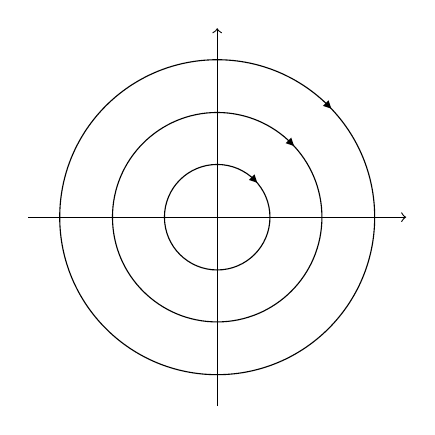
\begin{tikzpicture}
      \draw[->] (-2.4,0) -- (2.4,0);
      \draw[->] (0,-2.4) -- (0,2.4);
      \draw (0,0) circle (0.67);
      \fill[rotate=45] (0.67,-0.05) -- (0.72, 0.05) -- (0.62, 0.05) -- cycle;
      \draw (0,0) circle (1.33);
      \fill[rotate=45] (1.33,-0.05) -- (1.38, 0.05) -- (1.28, 0.05) -- cycle;
      \draw (0,0) circle (2.00);
      \fill[rotate=45] (2.00,-0.05) -- (2.05, 0.05) -- (1.95, 0.05) -- cycle;
    \end{tikzpicture}
  \end{figure}
\end{example}

\begin{theorem}
  Las trayectorias no se cortan.
  \begin{proof}
    Supongamos que las trayectorias asociadas a las soluciones \(x(t), y(t)\) de
    \(x' = Ax\) se cortan o, en otras palabras, que existen \(t_1, t_2\) tales
    que \(x(t_1) = y(t_2)\). Lo que ocurre es que \(y(t) = x(t + (t_1-t_2))\),
    luego la trayectoria que definen ambas soluciones resulta ser la misma.

    Para ver esto, definimos \(z(t) = x(t + (t_1-t_2))\). Se cumple que \(z' =
    Az\) y \(z(t_2) = x(t_1) = y(t_2)\), luego, en virtud del teorema de
    existencia y unicidad, debe ser \(z(t) = y(t)\).
  \end{proof}
\end{theorem}

\begin{remark}
  Ya vimos que las gráficas de \(x(t), y(t)\) no se cortan (como subconjuntos de
  \(\R^3\)). Este resultado, más fuerte, quiere decir que no se cortan \emph{sus
    proyecciones}, y se cumple porque \(A\) tiene coeficientes constantes (en
  caso contrario, no sería necesariamente cierto que \(z' = Az\)).
\end{remark}

\section{Interpretación geométrica de las trayectorias}

Una matriz \(A\), o más precisamente su aplicación lineal asociada \(A : \R^2
\to \R^2,\ x \mapsto Ax\), es un \emph{campo vectorial}. Una solución del
sistema \(x' = Ax\) no es más que una curva \(t \mapsto x(t)\) tal que su
velocidad \(x'(t)\) coincide con el valor del campo en \(x(t)\), es decir, una
\emph{curva integral} del campo.

\begin{example}
  Sea la matriz \(A = \smat{0 & 1 \\ -1 & 0}\). Esbozar el campo vectorial que
  define.

  La matriz \(A\) actúa sobre un vector genérico \(\smat{x_1 \\ x_2}\) como
  \(\smat{x_1 \\ x_2} \mapsto A\smat{x_1 \\ x_2} = \smat{x_2 \\ -x_1}\).
  Observamos que \(\langle x, Ax \rangle = 0\), es decir, la velocidad es
  ortogonal a la posición en todo punto, y además \(\|x\| = \|Ax\|\), es decir,
  \(A\) no cambia la norma de los vectores. El campo vectorial que define esta
  matriz es, entonces,

  \begin{figure}[ht]
    \centering
    \begin{tikzpicture}[scale=0.6]
      \draw[->] (-3.5,0) -- (3.5,0) node[above right] {\(x_1\)};
      \draw[->] (0,-3.5) -- (0,3.5) node[above right] {\(x_2\)};
      \foreach \r in {1, 2, 3}
      \foreach \a in {0,...,7}
      \draw[->] ({\r*cos(45*\a)}, {\r*sin(45*\a)}) --
      ({\r*cos(45*\a)+\r/2*sin(45*\a)}, {\r*sin(45*\a)-\r/2*cos(45*\a)});
    \end{tikzpicture}
  \end{figure}
\end{example}

\section{Representación gráfica de los sistemas planos}

Nos centramos ahora en esbozar el diagrama de fases de un sistema plano general
\(x' = Ax\), siendo \(B = P^{-1}AP\) su forma de Jordan. El cambio de variable
\(y = P^{-1}x\) transforma el sistema \(x' = Ax\) en \(y' = By\), mucho más
manejable. Las formas de Jordan posibles son

\begin{enumerate}[a)]
\item \(B = \smat{\lambda_1 & \\ & \lambda_2},\ \lambda_1 \neq \lambda_2\)
\item \(B = \smat{\lambda & \\ & \lambda}\)
\item \(B = \smat{\lambda & 1 \\ & \lambda}\)
\item \(B = \smat{a & b \\ -b & a},\ b>0\)
\end{enumerate}

Haremos los diagramas de fase para las formas de Jordan, y luego desharemos el
cambio de variable para obtener el diagrama final.

\subsection{Diagonalizable (dos autovalores distintos)}

Consideramos el sistema \(y' = \smat{\lambda_1 & \\ & \lambda_2} y\), con
\(\lambda_1 \neq \lambda_2\). Como hemos visto, la solución general del sistema
es

\[
  \begin{cases}
    y_1 = k_1e^{\lambda_1 t} \\
    y_2 = k_2e^{\lambda_2 t}
  \end{cases}
\]

Vamos a fijar distintos valores de \(k_1,k_2\) (i.e. distintos valores
iniciales) para ver cómo evoluciona el sistema a partir de ellos.

Empezamos por fijar valores sencillos, en los que algún valor inicial es 0
(valores iniciales en algún eje de coordenadas):

\begin{itemize}
\item \(k_1 = 0, k_2 = 0\): en este caso, la trayectoria es \(\{(0,0)\}\). Como
  consiste en un único punto, que permanece estable a lo largo del tiempo, se
  llama \emph{punto de equilibrio}.
\item \(k_1 > 0, k_2 = 0\): la trayectoria es \(\{(k_1e^{\lambda_1 t}, 0) : t \in
  \R\} = \{(y_1, 0) : y_1 > 0\}\)
\item \(k_1 < 0, k_2 = 0\): la trayectoria es \(\{(k_1e^{\lambda_1 t}, 0) : t \in
  \R\} = \{(y_1, 0) : y_1 < 0\}\)
\item \(k_1 = 0, k_2 > 0\): la trayectoria es \(\{(0, k_2e^{\lambda_2 t}) : t
  \in \R\} = \{(0,y_2) : y_2 > 0\}\)
\item \(k_1 = 0, k_2 < 0\): la trayectoria es \(\{(0, k_2e^{\lambda_2 t}) : t
  \in \R\} = \{(0,y_2) : y_2 < 0\}\)
\end{itemize}

En general, la trayectoria que pasa por el punto \(\smat{k_1 \\ k_2} \in \R^2\),
no necesariamente en algún eje, es
\(\{(k_1e^{\lambda_1 t}, k_2e^{\lambda_2 t}) : t \in \R\}\). Si el punto no está
sobre ninguno de los ejes, se cumple \(k_1 \neq 0 \neq k_2\), con lo que se
puede dividir entre ellos. Elevando la primera coordenada a \(\lambda_2\) y la
segunda a \(\lambda_1\), se tiene
\begin{equation}\label{eq:impl}
  \begin{cases}
    y_1^{\lambda_2} = k_1^{\lambda_2}e^{\lambda_1\lambda_2 t} \\
    y_2^{\lambda_1} = k_2^{\lambda_1}e^{\lambda_1\lambda_2 t}
  \end{cases} \implies \left(\frac{y_1}{k_1}\right)^{\lambda_2} = e^{\lambda_1
    \lambda_2 t} = \left(\frac{y_2}{k_2}\right)^{\lambda_1}.
\end{equation}

Como \(\lambda_1 \neq \lambda_2\), alguno de los dos tiene que ser distinto de
0; podemos suponer, sin pérdida de generalidad, que es \(\lambda_1\). Despejando
en \eqref{eq:impl}, llegamos a
\[y_2 = k_2 \left(\frac{y_1}{k_1}\right)^{\lambda_2 / \lambda_1}\]
es decir, una relación de la forma \(y_2 = c y_1^\alpha\). Distinguimos casos en
función del valor de \(\alpha\):

\begin{figure}[ht]
  \centering
  \begin{subfigure}{0.25\textwidth}
    \centering
    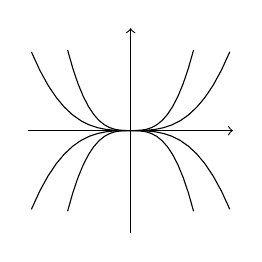
\begin{tikzpicture}
      \draw[->] (-1.3,0) -- (1.3,0);
      \draw[->] (0,-1.3) -- (0,1.3);
      \draw [domain=-1.26:1.26] plot (\x, {0.5*\x^3});
      \draw [domain=-1.26:1.26] plot (\x, {-0.5*\x^3});
      \draw [domain=-0.8:0.8] plot (\x, {2*\x^3});
      \draw [domain=-0.8:0.8] plot (\x, {-2*\x^3});
    \end{tikzpicture}
    \caption*{\(\alpha > 1\)}
  \end{subfigure}%
  \begin{subfigure}{0.25\textwidth}
    \centering
    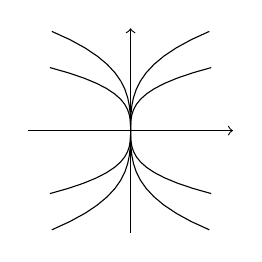
\begin{tikzpicture}
      \draw[->] (-1.3,0) -- (1.3,0);
      \draw[->] (0,-1.3) -- (0,1.3);
      \draw [domain=-1.26:1.26] plot ({0.5*\x^3}, \x);
      \draw [domain=-1.26:1.26] plot ({-0.5*\x^3}, \x);
      \draw [domain=-0.8:0.8] plot ({2*\x^3}, \x);
      \draw [domain=-0.8:0.8] plot ({-2*\x^3}, \x);
    \end{tikzpicture}
    \caption*{\(0 < \alpha < 1\)}
  \end{subfigure}%
  \begin{subfigure}{0.25\textwidth}
    \centering
    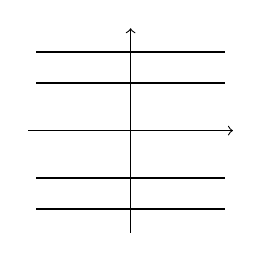
\begin{tikzpicture}
      \draw[->] (-1.3,0) -- (1.3,0);
      \draw[->] (0,-1.3) -- (0,1.3);
      \draw[thick] (-1.2,1) -- (1.2,1);
      \draw[thick] (-1.2,0.6) -- (1.2,0.6);
      \draw[thick] (-1.2,-0.6) -- (1.2,-0.6);
      \draw[thick] (-1.2,-1) -- (1.2,-1);
    \end{tikzpicture}
    \caption*{\(\alpha = 0\)}
  \end{subfigure}%
  \begin{subfigure}{0.25\textwidth}
    \centering
    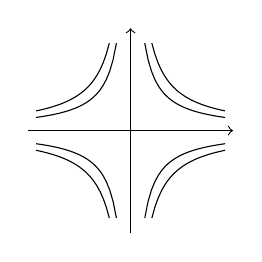
\begin{tikzpicture}
      \draw[->] (-1.3,0) -- (1.3,0);
      \draw[->] (0,-1.3) -- (0,1.3);
      \draw [domain=0.18:1.2] plot (\x, {0.2*\x^(-1)});
      \draw [domain=-1.2:-0.18] plot (\x, {0.2*\x^(-1)});
      \draw [domain=0.18:1.2] plot (\x, {-0.2*\x^(-1)});
      \draw [domain=-1.2:-0.18] plot (\x, {-0.2*\x^(-1)});
      \draw [domain=0.27:1.2] plot (\x, {0.3*\x^(-1)});
      \draw [domain=-1.2:-0.27] plot (\x, {0.3*\x^(-1)});
      \draw [domain=0.27:1.2] plot (\x, {-0.3*\x^(-1)});
      \draw [domain=-1.2:-0.27] plot (\x, {-0.3*\x^(-1)});
    \end{tikzpicture}
    \caption*{\(\alpha < 0\)}
  \end{subfigure}
\end{figure}

\begin{itemize}
\item Si \(\alpha < 0\), \(\lambda_1\) y \(\lambda_2\) tienen necesariamente
  signos opuestos. En este caso, el diagrama de fases (o más específicamente, el
  punto de equilibrio) recibe el nombre de \emph{punto de silla} (piénsese en
  las curvas de nivel de la función ``silla de montar'' \(z = x^2 - y^2\)).
\item Si \(\alpha > 0\), \(\lambda_1\) y \(\lambda_2\) tienen el mismo signo.
  \begin{itemize}
  \item Si es positivo, al aumentar \(t\) aumenta también la magnitud de la
    solución, es decir, se aleja (exponencialmente) del origen. Por esto, el
    diagrama (o el punto de equilibrio) recibe el nombre de \emph{nodo
      inestable}.
  \item Si es negativo, al aumentar \(t\) disminuye la magnitud de la solución,
    es decir, se acerca (exponencialmente) al origen. Por esto, el diagrama (o
    el punto de equilibrio) recibe el nombre de \emph{nodo estable}.
  \end{itemize}
  Hay que mencionar que el origen en sí siempre es una solución estable; estos
  nombres hacen referencia a lo que ocurre tras una desviación, por pequeña que
  sea, desde este punto.
\end{itemize}

Los demás casos los veremos con menos detalle, porque las ideas generales son
las mismas para todos y porque éste es el más delicado.

\subsection{Diagonalizable (un autovalor)}

Consideramos el sistema \(y' = \smat{\lambda & \\ & \lambda} y\). La solución
general es
\[
  \begin{cases}
    y_1 = k_1e^{\lambda t} \\
    y_2 = k_2e^{\lambda t}
  \end{cases}
\]
de donde \(y_1/k_1 = y_2/k_2 > 0\); esta es la ecuación de una semirrecta que
pasa por el origen (de hecho, coincide con el caso límite \(\alpha = 1\) en el
apartado anterior).

\begin{figure}[ht]
  \centering
  \begin{subfigure}{0.5\textwidth}
    \centering
    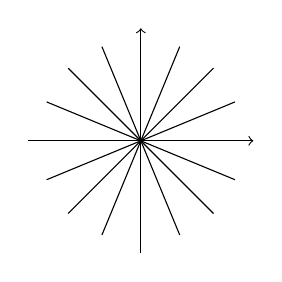
\begin{tikzpicture}[scale=1.3]
      \draw[->] (-1.1,0) -- (1.1,0);
      \draw[->] (0,-1.1) -- (0,1.1);
      \draw (-0.92, -0.38) -- (0.92, 0.38);
      \draw (0.92, -0.38) -- (-0.92, 0.38);
      \draw (-0.71, -0.71) -- (0.71, 0.71);
      \draw (0.71, -0.71) -- (-0.71, 0.71);
      \draw (-0.38, -0.92) -- (0.38, 0.92);
      \draw (0.38, -0.92) -- (-0.38, 0.92);
    \end{tikzpicture}
    \caption*{\(\lambda \neq 0\)}
  \end{subfigure}%
  \begin{subfigure}{0.5\textwidth}
    \centering
    \begin{tikzpicture}[scale=1.3]
      \draw[->] (-1.1,0) -- (1.1,0);
      \draw[->] (0,-1.1) -- (0,1.1);
      \foreach \x in {-0.92, -0.71, -0.38, 0, 0.38, 0.71, 0.92}
      \foreach \y in {-0.92, -0.71, -0.38, 0, 0.38, 0.71, 0.92}
      \fill (\x, \y) circle (0.5pt);
    \end{tikzpicture}
    \caption*{\(\lambda = 0\)}
  \end{subfigure}
\end{figure}

\begin{itemize}
\item Si \(\lambda > 0\), la solución se aleja (exponencialmente) del origen; el
  diagrama recibe el nombre de \emph{punto de estrella inestable}. Es un nodo
  inestable degenerado.
\item Si \(\lambda < 0\), la solución se acerca (exponencialmente) al origen; el
  diagrama recibe el nombre de \emph{punto de estrella estable}. Es un nodo
  estable degenerado.
\item Si \(\lambda = 0\), la solución es constante para cualquier valor inicial,
  es decir, el sistema no evoluciona con el tiempo.
\end{itemize}

\subsection{No diagonalizable (autovalor real)}
Consideramos el sistema \(y' = \smat{\lambda & 1 \\ & \lambda}y\), cuya solución
general es
\[
  \begin{cases}
    y_1 = (k_1+k_2t)e^{\lambda t} \\
    y_2 = k_2e^{\lambda t}
  \end{cases}
\]

Si \(\lambda = 0\), esta solución queda reducida a

\[
  \begin{cases}
    y_1 = k_1 + k_2 t \\
    y_2 = k_2
  \end{cases}
\]

La segunda coordenada permanece constante a lo largo del tiempo, mientras que la
primera varía desde \(-\infty\) hasta \(+\infty\) (si \(k_2 > 0\)) o desde
\(+\infty\) hasta \(-\infty\) (si \(k_2 < 0\)).

Si \(\lambda \neq 0\), distinguimos casos en función del valor inicial:

\begin{itemize}
\item \(k_1 = 0, k_2 = 0\): \(\{(0,0)\}\) es un punto de equilibrio
\item \(k_1 \neq 0, k_2 = 0\): los dos semiejes de abscisas
  \(\{(y_1, 0) : y_1 > 0\}\) y \(\{(y_1,0) : y_1 < 0\}\) son trayectorias
\item Si \(k_2 \neq 0\), podemos despejar \(t\) de \(y_2 = k_2e^{\lambda t}\) como
  \[t = \frac{1}{\lambda} \log \frac{y_2}{k_2}.\]

  Sustituyendo en \(y_1 = (k_1 + k_2t)e^{\lambda t}\), obtenemos una ecuación
  implícita para la trayectoria:
  \[y_1 = y_2 \left( \frac{k_1}{k_2} + \frac{1}{\lambda} \log \frac{y_2}{k_2}
    \right).\]

  Derivando implícitamente se obtiene
  \(\frac{\dif y_1}{\dif y_2} = \frac{\lambda y_1 + y_2}{\lambda y_2}\); esto
  quiere decir que, a lo largo de la recta \(\{y_2 = -\lambda y_1\}\), esta
  derivada se anula y, por tanto, las trayectorias tienen en esa recta tangente
  vertical.
\end{itemize}

Juntándolo todo, los diagramas de fase son

\begin{figure}[ht]
  \centering
  \begin{subfigure}{0.3\textwidth}
    \centering
    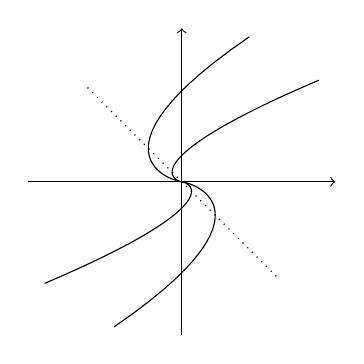
\begin{tikzpicture}[scale=1.5]
      \draw[->] (-1.3,0) -- (1.3,0);
      \draw[->] (0,-1.3) -- (0,1.3);
      \draw[samples=100, domain = -10:-0.15] plot ({(1.5 + \x)*exp(\x)}, {exp(\x)});
      \draw[samples=100, domain = -10:-0.15] plot ({(-1.5 - \x)*exp(\x)}, {-exp(\x)});
      \draw[samples=100, domain = -10:-0.2] plot ({(1 + 1.5*\x)*exp(\x)}, {1.5*exp(\x)});
      \draw[samples=100, domain = -10:-0.2] plot ({(-1 - 1.5*\x)*exp(\x)}, {-1.5*exp(\x)});
      \draw[thin, dotted] (0.8, -0.8) -- (-0.8, 0.8);
    \end{tikzpicture}
    \caption*{\(\lambda > 0\)}
  \end{subfigure}%
  \begin{subfigure}{0.3\textwidth}
    \centering
    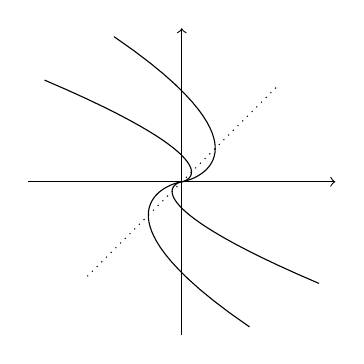
\begin{tikzpicture}[scale=1.5]
      \draw[->] (-1.3,0) -- (1.3,0);
      \draw[->] (0,-1.3) -- (0,1.3);
      \draw[samples=100, domain = 0.15:10] plot ({(1.5 - \x)*exp(-\x)}, {-exp(-\x)});
      \draw[samples=100, domain = 0.15:10] plot ({(-1.5 + \x)*exp(-\x)}, {exp(-\x)});
      \draw[samples=100, domain = 0.2:10] plot ({(1 - 1.5*\x)*exp(-\x)}, {-1.5*exp(-\x)});
      \draw[samples=100, domain = 0.2:10] plot ({(-1 + 1.5*\x)*exp(-\x)}, {1.5*exp(-\x)});
      \draw[thin, dotted] (-0.8, -0.8) -- (0.8, 0.8);
    \end{tikzpicture}
    \caption*{\(\lambda < 0\)}
  \end{subfigure}%
  \begin{subfigure}{0.3\textwidth}
    \centering
    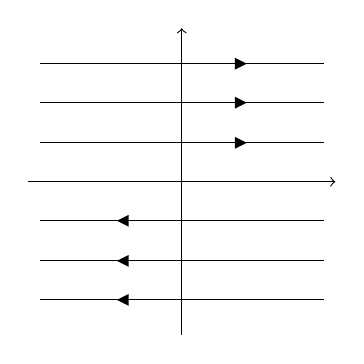
\begin{tikzpicture}[scale=1.5]
      \draw[->] (-1.3,0) -- (1.3,0);
      \draw[->] (0,-1.3) -- (0,1.3);
      \foreach \y in {1, 0.67, 0.33}
      {
        \draw (-1.2,\y) -- (1.2,\y);
        \fill (0.55, \y) -- (0.45, \y-0.05) -- (0.45, \y+0.05) -- cycle;
      }
      \foreach \y in {-0.33, -0.67, -1}
      {
        \draw (-1.2,\y) -- (1.2,\y);
        \fill (-0.55, \y) -- (-0.45, \y+0.05) -- (-0.45, \y-0.05) -- cycle;
      }
    \end{tikzpicture}
    \caption*{\(\lambda = 0\)}
  \end{subfigure}
\end{figure}

Como siempre, el comportamiento es distinto en función del signo de \(\lambda\):

\begin{itemize}
\item Si \(\lambda > 0\), la solución se aleja exponencialmente del origen. En
  este caso, el diagrama se llama \emph{nodo impropio inestable}.
\item Si \(\lambda < 0\), la solución se acerca exponencialmente al origen. En
  este caso, el diagrama se llama \emph{nodo impropio estable}.
\end{itemize}

\subsection{No diagonalizable (autovalores complejos)}
Consideramos el sistema \(y' = \smat{a & b \\ -b & a}y\), que tiene por solución
general

\[
  \begin{cases}
    y_1 = e^{at}(k_1 \cos bt + k_2 \sin bt) \\
    y_2 = e^{at}(-k_1 \sin bt + k_2 \cos bt)
  \end{cases}
\]

Definimos \(r_0^2 = k_1^2+k_2^2\) y \(\theta_0 \in \R\) tal que
\[\cos \theta_0 = \frac{k_1}{r_0} \qquad \text{y} \qquad \sin \theta_0 = \frac{k_2}{r_0}.\]
Se puede comprobar que así la solución general toma la forma
\[
  \begin{cases}
    y_1 = r_0e^{at} \cos (\theta_0 - bt) \\
    y_2 = r_0e^{at} \sin (\theta_0 - bt)
  \end{cases}
\]

y, definiendo \(r(t) = r_0e^{at}\) y \(\theta(t) = \theta_0 - bt\), se tiene
\[
  \begin{cases}
    y_1 = r(t) \cos \theta(t) \\
    y_2 = r(t) \sin \theta(t)
  \end{cases}
\]
con lo que queda descrito el camino \(t \mapsto \smat{y_1(t) \\ y_2(t)}\) en
coordenadas polares.

\begin{itemize}
\item Si \(a = 0\), entonces \(r(t) \equiv r_0\), es decir, las trayectorias son
  circunferencias de radio \(r_0\)
\item Si \(a \neq 0\), entonces las trayectorias son \emph{espirales logarítmicas}
\end{itemize}

\begin{figure}[ht]
  \centering
  \begin{subfigure}{0.5\textwidth}
    \centering
    \begin{tikzpicture}[scale=0.7]
      \draw[->] (-3,0) -- (3,0);
      \draw[->] (0,-3) -- (0,3);
      \draw [samples=100, domain = -10:1] plot ({exp(\x)*cos(-\x r)},{exp(\x)*sin(-\x r)});
      \draw [samples=100, domain = -10:1] plot ({exp(\x)*cos((2-\x) r)},{exp(\x)*sin((2-\x) r)});
      \draw [samples=100, domain = -10:1] plot ({exp(\x)*cos((4-\x) r)},{exp(\x)*sin((4-\x) r)});
    \end{tikzpicture}
    \caption*{\(a \neq 0\)}
  \end{subfigure}%
  \begin{subfigure}{0.5\textwidth}
    \centering
    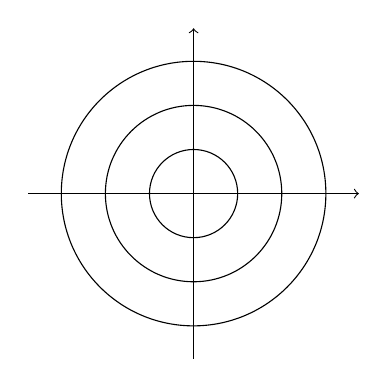
\begin{tikzpicture}[scale=0.7]
      \draw[->] (-3,0) -- (3,0);
      \draw[->] (0,-3) -- (0,3);
      \draw (0,0) circle (0.8);
      \draw (0,0) circle (1.6);
      \draw (0,0) circle (2.4);
    \end{tikzpicture}
    \caption*{\(a = 0\)}
  \end{subfigure}
\end{figure}

\begin{itemize}
\item Si \(\lambda > 0\), las soluciones se alejan exponencialmente del
  origen. En este caso, el diagrama recibe el nombre de \emph{foco inestable}.
\item Si \(\lambda < 0\), las soluciones se acercan exponencialmente al
  origen. En este caso, el diagrama recibe el nombre de \emph{foco estable}.
\end{itemize}

\subsection{Deshacer el cambio}
Habíamos hecho el cambio de variable \(y = P^{-1}x\) para resolver el sistema
\(x' = Ax = (PBP^{-1})x\). Ahora lo deshacemos: \(x = Py = \smat{v_1 & v_2}
\smat{y_1 \\ y_2}\).

Como ya sabemos de Álgebra Lineal, la transformaciones lineales
\(\R^2 \to \R^2\) no singulares deforman, rotan o hacen reflexiones sobre el
plano. Estas transformaciones quedan completamente determinadas por las imágenes de
dos vectores linealmente independientes, que en nuestro caso son \(e_1 = \smat{1
  \\ 0}\) y \(e_2 = \smat{0 \\ 1}\).

\(P\) es la \emph{única} transformación lineal que lleva \(e_1 \mapsto v_1\) y
\(e_2 \mapsto v_2\). Por tanto, para obtener el diagrama de fase de \(x' = Ax\),
basta transformar el de \(y' = By\) de forma que sea compatible con las
transformaciones
\[e_1 \mapsto v_1 \qquad e_2 \mapsto e_2.\]

\end{document}